\documentclass[aps,pra,twocolumn,superscriptaddress,floatfix]{revtex4-2}
 
\usepackage{amsmath,amssymb} % math symbols
\usepackage[english]{babel}
\usepackage{braket}%used for the \bra \ket notation
\usepackage{bm} % bold math font
\usepackage{caption}
	%\captionsetup{justification=raggedright,singlelinecheck=false}%force caption aligning to the left
\usepackage{comment} % allows block comments
\usepackage[ISO]{diffcoeff} %differentials and derivatives package
\usepackage{graphicx} % for figures
\usepackage[percent]{overpic}
\usepackage{pgfplots} % for figures
\usepgfplotslibrary{groupplots}
\usepackage{subcaption}	
\pgfplotsset{compat=1.16}
\usepackage{textcomp} % This package is just to give the text quote '
\usepackage{tikz}
%\usepackage{ulem} % allows strikeout text, e.g. \sout{text}
\usepackage{enumitem}
\setlist{noitemsep,leftmargin=*,topsep=0pt,parsep=0pt}

\usepackage{xcolor} % \textcolor{red}{text} will be red for notes
\definecolor{lightgray}{gray}{0.6}
\definecolor{medgray}{gray}{0.4}

\newcommand\Ga
{\mathbf{\Gamma}}
\usepackage{hyperref}
\hypersetup{
colorlinks=true,
urlcolor= blue,
citecolor=blue,
linkcolor= blue,
% bookmarks=true,
% bookmarksopen=false,
}

\newcommand{\mytitle}{Design of Bent Waveguide Via Shortcuts to Adiabaticity}

\usepackage{cleveref}
\begin{document}
\title{\mytitle}
\author{Manuel Odelli, Andreas Ruschhaupt}
\affiliation{UCC College Cork}
\begin{abstract}
Waveguides are one of the  key components in the design and developement of quantum computers as they channel the information between computational sites.
With the size of quantum chips continuously reducing, it is necessary to devise new strategies to meet these geometrical constraints, but at the same time ensuring the trasmission of information is lossless and stable.
One of the most common and widespread purpose of waveguides is to allow a particle to be transmitted around a corner to connect two straight ends with ideally no reflection rates.
The easiest solution to this problem has been to increase the strength of the trapping.
This approach, however, requires a great amount of energy and it would be preferrable to rely on a strategy primarily aiming to affect the geometry of the waveguide allowing for the intensity of the trapping frequency to be reduced. 
The aim of this paper is to further improve on existing protocol based on Shortcuts to Adiabaticity and to highlight how purely geometrical effects can affect its fidelity.
\end{abstract}
\maketitle

\section{Introduction}
The advancements of quantum technologies in  recent years have brought the focus of the scientific community on the need to investigate novel approaches to produce more compact and stable quantum devices.
While the progressive miniaturisation of the devices poses geometrical constraints on the system, an optimal level of control on the quantum particles is required.
Waveguides in particular play a crucial role in the confinement and transmission of quantum states in a wide variety of experiments where the control is usually achieved by increasing the intensity of the trapping.
This approach is clearly energy consuming so it would be advisable to design protocols relying primarily on the geometry of the waveguide and only subsequently focusing on the strength of the trapping.
The effects of the geometry on waveguides are well known and could be quite disrupting as - for example - it has been shown that even the slightest bending in waveguides results in the production of bound states \cite{BoundStatesInGoldst1992}.
Historically, studies relied on the adiabatic approximation, by virtue of which the curvature is supposed to vary gently.
The adiabatic approximation is ineffective in those systems where strong geometrical constraints are in place as, for instance waveguides with sharp bendings \cite{BoundStatesInClark1996, BoundStatesInBittne2013, MultipleBoundCarini1993}.
Recently, the surge of inverse engineered protocols under the name of Shortcuts to Adiabaticity  \cite{ShortcutsToAdGuery2019} (STA) has proven to be extremely effective in systems where the adiabatic approach is deemed to be unapplicabile.
STA offer a framework to control the evolution of a system starting in some initial state to obtain the desired final state by ensuring that selected external parameters meet the boundary conditions.
In the context of waveguides, Gu\'ery-Odelin et al. in the seminal paper \cite{QuantumControlImpens2020} have applied the approach based on STA to design the curvature of sharply bent waveguides to minimise the loss of coherence in travelling quantum particles with excellent results.
The range of applicability of this protocol extends to all systems where matter-wave circuits are employed.
One of the most relevant example of application is atomtronics \cite{RoadmapOnAtomAmico2021}, an emerging field where the information carriers are cold neutral atoms and the applications of which span from quantum interferometry \cite{MagneticallyGuQiLu2017, 80kmomentumSeMcdona2013} to quantum circuital elements \cite{FocusOnAtomtrAmico2017, AdvancesInAtoPepino2021}.
The approach in \cite{QuantumControlImpens2020} is based on the assumption that - in first approximation - a quantum particle can be modelled as a classical one and that by imposing the trajectory it is possible to inverse engineer the curvature satisfying the boundary conditions.
In this paper we will first briefly review the STA-based approach of Gu\'ery-Odelin et al. and we subsequently change the controlling parameters to further investigate the validity of the protocol when the classical approximation loses its validity.
\section{Hamiltonian of a bent waveguide}
Let us consider a system composed by a waveguide where the confinement is achieved by means of a harmonic trapping of intensity $ \omega $.
With no loss of generality, we can assume that the waveguide is formed by two straight ducts forming an angle $\alpha = \pi/2$ and connected by a bent section.
We also assume that the initial state is a separable 2D Gaussian wave packet entering the curved trait with momentum $k_0$, and hence it can be written as 
\begin{align}
\label{eq:initial_state}
	\psi_{0}(x,y) = \left(\frac{1}{2 \pi \sigma_{x}^{2}}\right)^{1/4}\exp\left(- \frac{x^{2}}{4\sigma_{x}^{2}} - i k_{0}x  \right)\\
	\left(\frac{1}{2\pi\sigma_{y}^{2}}\right)^{1/4}\exp\left(-\frac{y^{2}}{4\sigma_{y}^{2}}\right)
\end{align}
where $ \sigma_{y} $  is the dispersion along the transverse axis equal to $\sqrt{\hbar/2 m \omega}$ while the longitudinal dispersion $ \sigma_{x} $ is set.
If no bending was involved, $\psi_0$  would evolve under the effect of the Hamiltonian of a straight waveguide 
\begin{equation}
	\label{eq:straightwave}
	 H = -\frac{\hbar^2}{2m} \left(\partial_{x}^{2} + \partial_{y}^{2}\right) + \frac{1}{2}m\omega^2y^2
\end{equation}
and we could write the wave function at the time $t$ as the product of a free particle along $x$ and the ground state of the harmonic oscillator along $y$. 
On the other hand, if we assume the waveguide to be bent and considering the bottom of the trap to follow a curve $\Ga$ in $\mathbb{R}^2$, the modification in the geometry of the system produces mixing between the two components of the wave function, hence making harder it to control the particle.
The Hamiltonian of this system has been studied extensively in the literature (see for example \cite{TheEffectiveHKrejci2012}) and can be evaluated by using the most convenient curvilinear coordinates $(s,u)$ where $s$ is defined as the arc length of $\Ga$ defined as $s(t) = \int_0^t d\tau||\Ga'(\tau)||$ and $u$ is the transverse coordinate.
The local coordinate axis are the normal vectors \textbf{t}(s), \textbf{n}(s), with \textbf{t} the tangent vector to the curve and \textbf{n} the unit vector perpendicolar to \textbf{t} as in  \cref{fig:setup}.
\begin{figure}
	%(a)	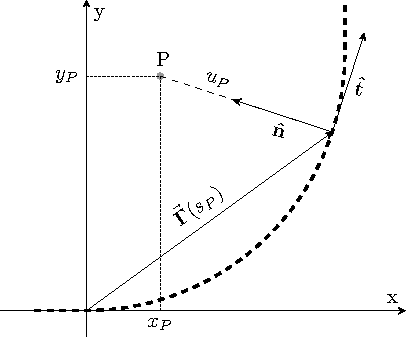
\includegraphics[width = .7\columnwidth]{gfx/frenet.pdf}\\
		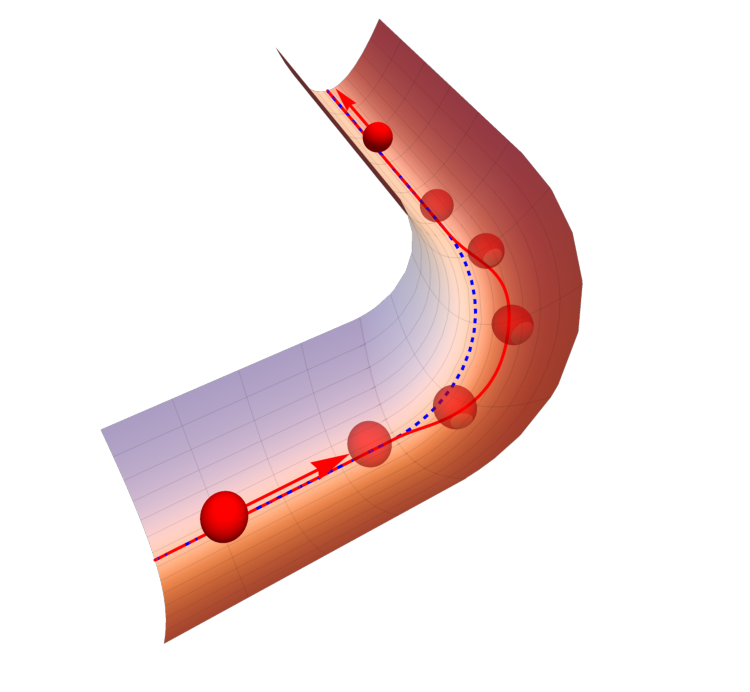
\includegraphics[width = .7\columnwidth]{gfx/tube.pdf}
		\caption{%(a) Schematic to show the construction of the Frenet Serrat frame of reference and how the curvilinear coordinates are defined.\\
		 Example of the imposed trajectory of the particle in a waveguide with harmonic trapping}
		\label{fig:setup}
\end{figure}
With this prescriptions, the coordinate transformation from Cartesian coordinates to the so-called Frenet Serrat frame can be written as $(x(s,u), y(s,u)) = \Ga(s)  + u \mathbf{n}(s) $ as in \cref{fig:setup}.
Moreover, the following relations hold and they are called Frenet Serrat equations:
\begin{align}
	\diff{\Ga(s)}{s}  &= \mathbf{t}(s) \label{eq:frenet1}\\ 
	\diff{\mathbf{t}(s)}{s}  &= \gamma(s)\mathbf{n}(s) \label{eq:frenet2}\\ 
	\diff{\mathbf{n}(s)}{s}  &= -\gamma(s)\mathbf{t}(s) \label{eq:frenet3}
\end{align}
where $\gamma(s)$ is the curvature of $\Ga$ and it is invariant under transformation.
The curvature $\gamma$ is the most relevant quantity in this case since the Hamiltonian of the system can be written as 
\begin{equation}
	\label{eq:curvedhamilton}	
	H = - \frac{\hbar^2}{2m} \left( \partial_s \frac{1}{(1-\gamma)^2} - \partial_{u}^{2}\right)
	+ \frac{1}{2} m\omega^2u^2 + V(s,u)
\end{equation}
where $V(s,u)$ is the attractive potential resulting from the change of coordinates 
\begin{equation}
	\label{eq:potential}
	V(s,u) = -\frac{\gamma^2}{4(1-u\gamma)^2} - \frac{u\ddot{\gamma}}{2(1-u\gamma)^3} -\frac{5}{4}\frac{u^2\dot{\gamma}^2}{(1-u\gamma)^4}.
\end{equation}
In many studies an adiabatic approach has been followed to solve the Hamiltonian \eqref{eq:curvedhamilton} 
Adiabatic in the sense that the curvature has been chosen to be varying slowly with respect ot the $s$ coordinate, i.e. $\dot{\gamma}, \ddot{\gamma} \approx 0 $.
This approach does not take into account many particular settings, for example the ones with geometric consstraints where a sharp turn needs to be considered.
For this reason Gu\'ery-Odelin et al in \cite{QuantumControlImpens2020} have designed a semi-classical protocol based on Shortcuts to Adiabaticity (STA) to circumvent the limitations of the adiabatic approach.
In \cite{QuantumControlImpens2020} the curvature $\gamma$ has been inversed engineered by writing the classical 2D Newton's equations of motion for a particle with initial speed $\dot{s}_0$.
The idea is to impose the dependence of the curvature coordinates $(s,u)$ from the time parameter $t$ so that the position of a point particle of mass $m$ can be described bt the vector $\Ga(s(t))$.
We can hence write the respective Newton's equation in vector form as 
\begin{equation}
	\label{eq:newtfirstlaw}
	m \diff[2]{\Ga(s(t))} t = - \nabla V_\perp (u)
\end{equation}
where $ V_\perp(u) $ is the conservative trapping potential that in curvilinear coordinates simply becomes $ \frac{1}{2}\omega^2 u^2 $.
The solution of \eqref{eq:newtfirstlaw} is obtained by making use of \crefrange{eq:frenet1}{eq:frenet3} and projecting the resulting vector onto the two coordinate axis \textbf{t} and \textbf{n}:
\begin{align}
	& \ddot{s} (1-u\gamma)  -\dot{s}(2\dot{u}\gamma + u \dot{\gamma}) + \frac{1}{2}\omega^2u^2 = 0 \\
	& \ddot{u} + \omega^2u + \dot{s}^2\omega(1-u\gamma)  = 0.
\end{align}
Furthermore, the conservation of energy can be written as $\frac{1}{2}\left(\diff{\Ga}{t}\right)^2 + V_\perp(s,u) = E$ or, equivalently
\begin{equation}
	\label{eq:energyconserve}
	\dot{u}^2 + \omega^2u^2 + \dot{s}^2(1-u\gamma)^2 = \dot{s}_0^2.
\end{equation}
By setting $ v_\gamma = \dot{s}(1-u\gamma)   $, it has been shown that it is possible to retrieve $ \gamma $ using the following formula
\begin{equation}
	\label{eq:stacurvature}
	\gamma = \frac{\dot{v}_\gamma}{\diff{}{t}(uv_\gamma)}	,
\end{equation}
hence the curvature can be obtained only by fixing the transverse trajectory $ u_{sta}(t) $ as exemplified in \cref{fig:setup}.
The resulting curvature $ \gamma_{sta} $ can then be used as the groundwork to numerically solve the Hamiltonian \eqref{eq:curvedhamilton} and thest the performances of the waveguide's geometry also in quantum settings.
It has already been shown in \cite{QuantumControlImpens2020} that a curve obtained following this procedure provides a higher level of fidelity when  compared to a circular waveguide of radius $R$.
In the following we will try ot continue on these tracks by testing different transverse trajectories.

\section{Hamiltonian of a bent waveguide}
Let us consider a system composed by a waveguide where the confinement is achieved by means of a harmonic trapping of intensity $ \omega $.
With no loss of generality, we can assume that the waveguide is formed by two straight ducts forming an angle $\alpha = \pi/2$ and connected by a bent section.
We also assume that the initial state is a separable 2D Gaussian wave packet entering the curved trait with momentum $k_0$, and hence it can be written as 
\begin{align}
\label{eq:initial_state}
	\psi_{0}(x,y) = \left(\frac{1}{2 \pi \sigma_{x}^{2}}\right)^{1/4}\exp\left(- \frac{x^{2}}{4\sigma_{x}^{2}} - i k_{0}x  \right)\\
	\left(\frac{1}{2\pi\sigma_{y}^{2}}\right)^{1/4}\exp\left(-\frac{y^{2}}{4\sigma_{y}^{2}}\right)
\end{align}
where $ \sigma_{y} $  is the dispersion along the transverse axis equal to $\sqrt{\hbar/2 m \omega}$ while the longitudinal dispersion $ \sigma_{x} $ is set.
If no bending was involved, $\psi_0$  would evolve under the effect of the Hamiltonian of a straight waveguide 
\begin{equation}
	\label{eq:straightwave}
	 H = -\frac{\hbar^2}{2m} \left(\partial_{x}^{2} + \partial_{y}^{2}\right) + \frac{1}{2}m\omega^2y^2
\end{equation}
and we could write the wave function at the time $t$ as the product of a free particle along $x$ and the ground state of the harmonic oscillator along $y$. 
On the other hand, if we assume the waveguide to be bent and considering the bottom of the trap to follow a curve $\Ga$ in $\mathbb{R}^2$, the modification in the geometry of the system produces mixing between the two components of the wave function, hence making harder it to control the particle.
The Hamiltonian of this system has been studied extensively in the literature (see for example \cite{TheEffectiveHKrejci2012}) and can be evaluated by using the most convenient curvilinear coordinates $(s,u)$ where $s$ is defined as the arc length of $\Ga$ defined as $s(t) = \int_0^t d\tau||\Ga'(\tau)||$ and $u$ is the transverse coordinate.
The local coordinate axis are the normal vectors \textbf{t}(s), \textbf{n}(s), with \textbf{t} the tangent vector to the curve and \textbf{n} the unit vector perpendicolar to \textbf{t} as in  \cref{fig:setup}.
\begin{figure}
	%(a)	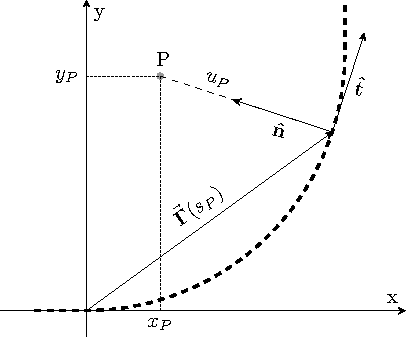
\includegraphics[width = .7\columnwidth]{gfx/frenet.pdf}\\
		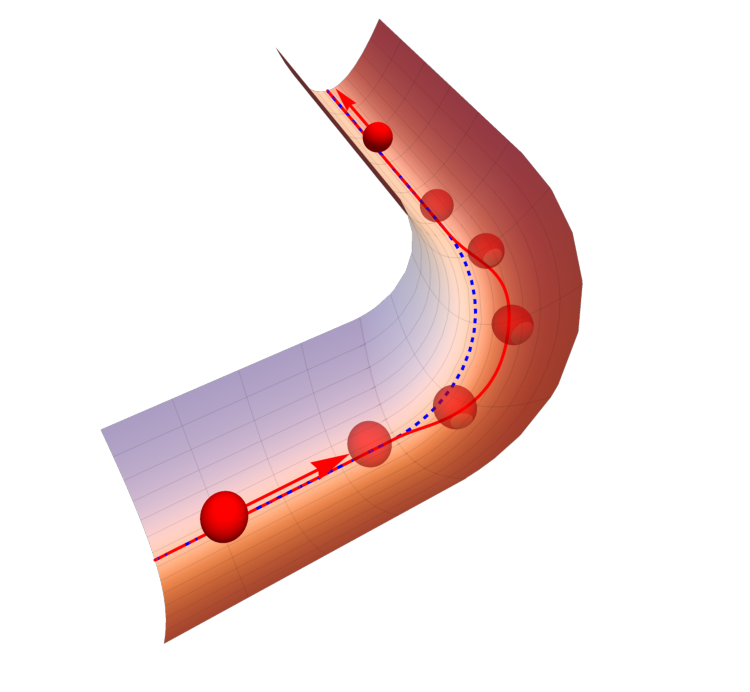
\includegraphics[width = .7\columnwidth]{gfx/tube.pdf}
		\caption{%(a) Schematic to show the construction of the Frenet Serrat frame of reference and how the curvilinear coordinates are defined.\\
		 Example of the imposed trajectory of the particle in a waveguide with harmonic trapping}
		\label{fig:setup}
\end{figure}
With this prescriptions, the coordinate transformation from Cartesian coordinates to the so-called Frenet Serrat frame can be written as $(x(s,u), y(s,u)) = \Ga(s)  + u \mathbf{n}(s) $ as in \cref{fig:setup}.
Moreover, the following relations hold and they are called Frenet Serrat equations:
\begin{align}
	\diff{\Ga(s)}{s}  &= \mathbf{t}(s) \label{eq:frenet1}\\ 
	\diff{\mathbf{t}(s)}{s}  &= \gamma(s)\mathbf{n}(s) \label{eq:frenet2}\\ 
	\diff{\mathbf{n}(s)}{s}  &= -\gamma(s)\mathbf{t}(s) \label{eq:frenet3}
\end{align}
where $\gamma(s)$ is the curvature of $\Ga$ and it is invariant under transformation.
The curvature $\gamma$ is the most relevant quantity in this case since the Hamiltonian of the system can be written as 
\begin{equation}
	\label{eq:curvedhamilton}	
	H = - \frac{\hbar^2}{2m} \left( \partial_s \frac{1}{(1-\gamma)^2} - \partial_{u}^{2}\right)
	+ \frac{1}{2} m\omega^2u^2 + V(s,u)
\end{equation}
where $V(s,u)$ is the attractive potential resulting from the change of coordinates 
\begin{equation}
	\label{eq:potential}
	V(s,u) = -\frac{\gamma^2}{4(1-u\gamma)^2} - \frac{u\ddot{\gamma}}{2(1-u\gamma)^3} -\frac{5}{4}\frac{u^2\dot{\gamma}^2}{(1-u\gamma)^4}.
\end{equation}
In many studies an adiabatic approach has been followed to solve the Hamiltonian \eqref{eq:curvedhamilton} 
Adiabatic in the sense that the curvature has been chosen to be varying slowly with respect ot the $s$ coordinate, i.e. $\dot{\gamma}, \ddot{\gamma} \approx 0 $.
This approach does not take into account many particular settings, for example the ones with geometric consstraints where a sharp turn needs to be considered.
For this reason Gu\'ery-Odelin et al in \cite{QuantumControlImpens2020} have designed a semi-classical protocol based on Shortcuts to Adiabaticity (STA) to circumvent the limitations of the adiabatic approach.
In \cite{QuantumControlImpens2020} the curvature $\gamma$ has been inversed engineered by writing the classical 2D Newton's equations of motion for a particle with initial speed $\dot{s}_0$.
The idea is to impose the dependence of the curvature coordinates $(s,u)$ from the time parameter $t$ so that the position of a point particle of mass $m$ can be described bt the vector $\Ga(s(t))$.
We can hence write the respective Newton's equation in vector form as 
\begin{equation}
	\label{eq:newtfirstlaw}
	m \diff[2]{\Ga(s(t))} t = - \nabla V_\perp (u)
\end{equation}
where $ V_\perp(u) $ is the conservative trapping potential that in curvilinear coordinates simply becomes $ \frac{1}{2}\omega^2 u^2 $.
The solution of \eqref{eq:newtfirstlaw} is obtained by making use of \crefrange{eq:frenet1}{eq:frenet3} and projecting the resulting vector onto the two coordinate axis \textbf{t} and \textbf{n}:
\begin{align}
	& \ddot{s} (1-u\gamma)  -\dot{s}(2\dot{u}\gamma + u \dot{\gamma}) + \frac{1}{2}\omega^2u^2 = 0 \\
	& \ddot{u} + \omega^2u + \dot{s}^2\omega(1-u\gamma)  = 0.
\end{align}
Furthermore, the conservation of energy can be written as $\frac{1}{2}\left(\diff{\Ga}{t}\right)^2 + V_\perp(s,u) = E$ or, equivalently
\begin{equation}
	\label{eq:energyconserve}
	\dot{u}^2 + \omega^2u^2 + \dot{s}^2(1-u\gamma)^2 = \dot{s}_0^2.
\end{equation}
By setting $ v_\gamma = \dot{s}(1-u\gamma)   $, it has been shown that it is possible to retrieve $ \gamma $ using the following formula
\begin{equation}
	\label{eq:stacurvature}
	\gamma = \frac{\dot{v}_\gamma}{\diff{}{t}(uv_\gamma)}	,
\end{equation}
hence the curvature can be obtained only by fixing the transverse trajectory $ u_{sta}(t) $ as exemplified in \cref{fig:setup}.
The resulting curvature $ \gamma_{sta} $ can then be used as the groundwork to numerically solve the Hamiltonian \eqref{eq:curvedhamilton} and thest the performances of the waveguide's geometry also in quantum settings.
It has already been shown in \cite{QuantumControlImpens2020} that a curve obtained following this procedure provides a higher level of fidelity when  compared to a circular waveguide of radius $R$.
In the following we will try ot continue on these tracks by testing different transverse trajectories.

\section{Inverse Engineering Approach}
 It is clear from equation \eqref{eq:stacurvature} that the choice of $ u_{sta} $ is crucial to guarantee the stability of the protocol over a wide range of initial velocities and to ensure that the outcoming particle does not experience any kind of transverse excitation (as in \cref{fig:setup}) after the bent section.
 In particular, for a total travel time $ 2T $, the following constraints have been set:
 \begin{align}
 &	u_{sta}(0) =\dot{u}_{sta}(0) = \ddot{u}_{sta}(0) = 0 , \label{eq:boundary0}\\
 &	u_{sta}(T) = \Delta u_{sta}, \hspace{3em } \dot{u}_{sta}(T) = \ddot{u}_{sta}(T) = 0, \label{eq:boundary1}\\
 &	u_{sta}(2T) =\dot{u}_{sta}(0) = \ddot{u}_{sta}(0) = 0, \label{eq:boundary2}
 \end{align}
 where $ \Delta u_{sta} $ is the maximum transverse displacement in the middle of the curve and it is fixed by the physics of the system.
 A natural choice for $u_{sta}$ is a polynomial fulfilling the \crefrange{eq:boundary0}{eq:boundary2}.
 In \cite{QuantumControlImpens2020} the symmetry of the problem has been  exploited  by using $ u_{sta}(t)  = P(t/T)$ for the first section (i.e. for $ t \in [0,T]$) and the polynomial $ P(2-t/T) $ for $ t \in [T,2T] $ .
 Following the constraints of \crefrange{eq:boundary0}{eq:boundary2}, Gu{\'e}ry et al. choice for the polynomial is 
 \begin{equation}
	 \label{eq:order1poly}
 	P(\tau) = \Delta u_{sta}(10\tau^3 - 15\tau^4 + 6\tau^5) 
 \end{equation}
The resulting curvature presents a cusp in the centre of the path, due to the fact that the trajectory was defined on the half interval.
\begin{figure}
	\centering
		\begin{overpic}[scale = 1]{gfx/curves.pdf}
			\put(17,34){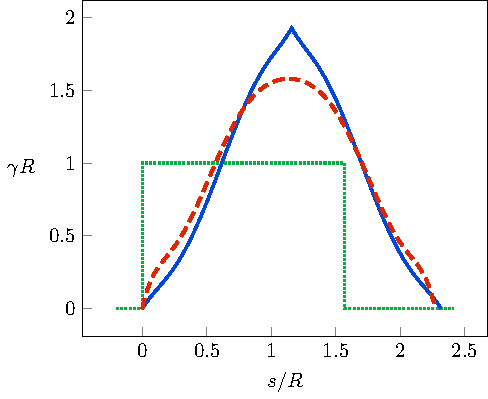
\includegraphics[scale = .55]{gfx/curvatures.pdf}}
		\end{overpic}
	\caption{View from the top of the curves for different $ n $. in this case $ k_{0}R = 500 $ and $ \omega T = 5 $.
	In the inset the comparison of different curvatures obtained by  setting different $ n $ is shown. We can see that for $ n \neq 1 $ the curvatures are smooth function witn cusps for $ t = T $ }
	\label{fig:curves}
	\caption{}
	\label{fig:curvatures}
\end{figure}
This may cause numerical instabilities and therefore we decided to use different trajectories defined on the whole interval $ [0,2T] $ and we will refer to them with the notation $U(t)$.
Moreover, we imposed the derivatives in \crefrange{eq:boundary0}{eq:boundary2} to be 0 up to the $ n^{th} $ order, so we can rewrite the boundary conditons are
\begin{align}
&	U^{(i)}(0) = 0 ~ \mathrm{for} ~  i = 0, ..., n, \\
&	U^{(0)}(T) = \Delta U, ~ U^{(i)(T)}=0 ~ \mathrm{for} ~ i = 1, ..., n, \\
&	U^{(i)}(2T) = 0 ~ \mathrm{for} ~ i = 0, ..., n.
\end{align}
We then tested the protocol for different $ n $ and we would like to remark that for each $n$ we evaluated the corresponding $ \Delta U_{n}  $ and $ T_{n} $.
In the remainder of the work we will identify every trajectory by the number $ n $ and to keep the notation consistent we will refer to $ u_{sta} $ as $ U_{1} $.
We will do the same for the curvature $ \gamma_{n} $ and the corresponding $ \Ga_{n} $. 
In \cref{fig:curvatures} we can see how the resulting curvatures are smoother functions and do not show any cusps in the middle.
Using the curvatures obtained applying the STA approach with different trajectories, we are now ready to simulate the evolution of the quantum state under the effects of the corresponding Hamiltonian.

\section{Numerical Simulation}
The quantum simulation has been carried out via the split operator method \cite{NoneFeit1982}, relying on the Fourier transform in cartesian coordinates.
Hence, the Frenet Serrat differential equations \crefrange{eq:frenet1}{eq:frenet2} have been solved to retrieve the curves $ \Ga_{n} $ (as in \cref{fig:curvatures}) and they have subsequently been used to build the potential in cartesian coordinates to rewrite the Hamiltonian \cref{eq:curvedhamilton} in the Cartesian frame of reference
\begin{equation*}
	\label{eq:splitophamilton}
	H = -\frac{\hbar^{2}}{2m}\left(\partial_{x}^{2}-\partial_{y}^{2}\right) + V_{C}(x,y)
\end{equation*}
where now $ V_{C}(x,y) $  is the whole potential in Cartesian coordinates, encompassing both the attractive potential $ V(s,u) $ due to the bending and the harmonic trapping $ V_{\perp}(u) $ of \cref{eq:curvedhamilton}.
We then choose the initial wave function $ \psi_{0} $ to be a travelling 2D Gaussian wave packet with initial momentum $ k_{0} $ in a harmonic waveguide of trapping frequency $ \omega $ as in \cref{eq:initial_state}.
Moreover, the longitudinal and transverse dispersion $ \sigma_{x} $  and $ \sigma_{y} $ have been fixed to 0.05 and $ \frac{1}{2} m\omega $ respectively.
Finally, the mass have been set to $ m = 400\hbar T/R^{2} $.
We will then simulate the time evolution of $ \psi_{0} $ \cref{eq:initial_state}  under the effect of the potential $ V_{C}(x,y) $, to obtain the final state $ \psi_{so} $.
To find the fidelity of this protocol we need to define a reference case, assumed to be ideal. 
In an ideal situation the wave function would evolve as if it was moving along a straight waveguide, hence no mixing between the longitudinal and transverse components would arise.
We refer to this reference wave function as $ \psi_{f} $ and we will evaluate the overlap with $ \psi_{so} $ to finally define the fidelity
\begin{equation}
	\label{eq:fidelity}
	F = |\braket{\psi_{f}|\psi_{so}}|^{2}.
\end{equation}
This approach is based on the assumption that - in first approximation - a quantum particle can be modelled as a classical one and this assumption has been proven to be effective and to yield high level of fidelity ($>99\%$).
But if we really want to compare the effects of the geometry on the fidelity for different curves $ \Ga_{n} $, the variables $ k_{0} $ and $ \omega $ need to be set in order to make the geometry of the system predominant with respect to the other properties.
With this in mind, we have decided to run the simulations for $ \omega T = 3,5,7 $ while the initial momentum has been varied until a significant drop in fidelity is reached and in the next section we will show and explain the results of our calculations.

\section{Results}
We have initially evaluated the fidelity for different $ n $ for a fixed trapping $ \omega $ and we progressively increased the initial speed $ k_{0} $ until a consistent drop in fidelity was met.
We can clearly see that the curve $ \Ga_{2} $ provides the higher level of fidelity for each different $ \omega $ and it is hence preferrable.
In addition, we note that the spectrum of velocities upon which the protocol is reliable gets wider as the strength of the transverse confinment increases, as predictable.
We then decided to compare the probability density of each wave packet in the straight end after the bent section to assess the deformation of the wave function due to the bending of the waveguide, as opposed to the ideal one and once again we could see how the mixing between transverse and longitudinal components is lower for $ n = 2 $ and that is reflected in a higher level of fidelity.
\begin{figure*}[t!]
	\centering
	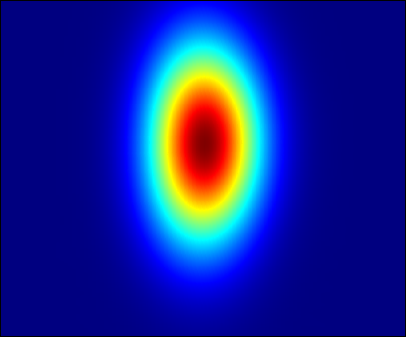
\includegraphics[width = .3\textwidth]{gfx/texdens_ord2_300_7.pdf}
	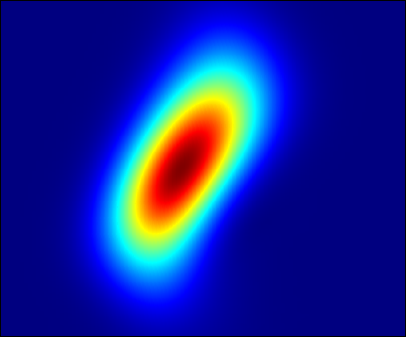
\includegraphics[width = .3\textwidth]{gfx/texdens_ord0_300_7.pdf}
	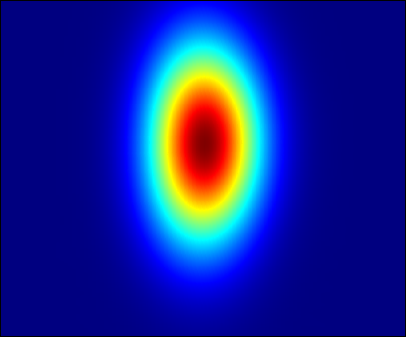
\includegraphics[width = .3\textwidth]{gfx/texdens_ord2_300_7.pdf}
	\caption{arison between the wave function density for different orders 1 to 4 (fig. (a) to (d) for $ \omega T = 7 $ and $ k_{0}R = 1100 $ with the corresponding fidelity. In fig.(a) the the mixing of the two components is more visible than the others and it is reflected in the value of the fidelity}
	\label{fig:densities}	
\end{figure*}
\begin{figure*}[t!]
		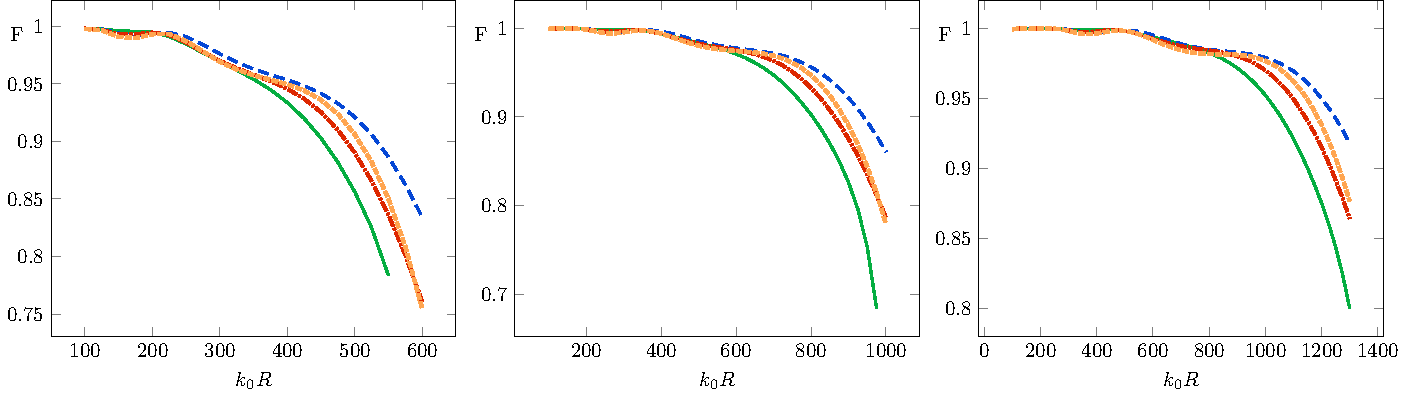
\includegraphics[width = \textwidth]{gfx/fidelities.pdf}
	\caption{Comparison of different fidelities for $ \omega = 3,5,7 $ where the initial momentum $ k_{0} $ varying until a consistent drop in the fidelity was reached. In all the three cases, we can see how the curve obtained for $ n = 2 $ is the one showing the best performances}
	\label{fig:fidelities}
\end{figure*}
Finally, we tested the robustness of each curve for different $ n $ and various speed.
The robustness against dispersion of velocity has been evaluated first by obtaining the curve for a fixed $ k_{0} $ known to ensure the best performances, and then used the same curve to simulate the time evolution of particles with initial velocity included in  $[ k_{0}  -  \epsilon,k_{0}  +  \epsilon]  $ and getting the corresponding fidelity as a function of the inital velocity.
We then defined the robustness as the second derivative of the fidelity with respect to the momentum and repeated this procedure for several $ k_{0} $ and for different $ n $.
The results are summarized in \cref{fig:robustness} and again we can observe that the curve $ \Ga_{2} $ is the one that provides the best performances.
\begin{figure}
	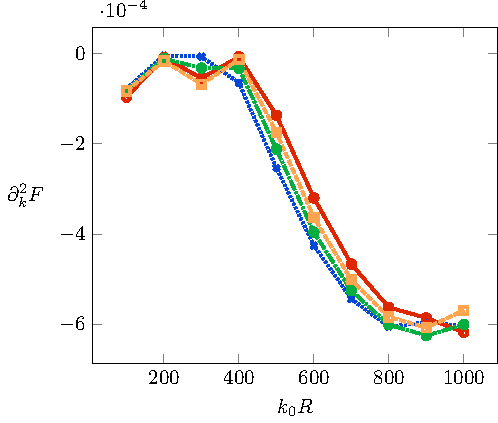
\includegraphics{gfx/robustness.pdf}
	\caption{Plot outlining the robustness for different curves for fixed $ \omega = 7 $ and for different velocities $ k_{0} $. The robustness is defined as the second derivative of the fidelity with respect to the initial momentum and again the best results are obtained for $ n = 2 $ }
	\label{fig:robustness}
\end{figure}

\bibliography{sections/bibliography.bib}

\end{document}
